\section{Case Study: 200 Nodes}
\subsection{Introduction}
In this chapter we want to analyze the case at 200 nodes, as it is the quantity that is halfway between our configurations. At the end of the simulations we decided to calculate the average coverage rate, summarized in this table.

\begin{table}[h!]
\centering
\begin{tabular}{|c|c|c|c|c|c|}
\hline
       & r=10    & r=30    & r=50    & r=75    & r=100   \\ \hline
p=0,15 & 0,90727 & 1       & 1       & 1       & 1       \\ \hline
p=0,3  & 0,89379 & 0,99924 & 0,99561 & 1       & 0,99924 \\ \hline
p=0,5  & 0,79909 & 0,99424 & 0,98803 & 0,98894 & 0,99591 \\ \hline
p=0,7  & 0,71045 & 0,97985 & 0,96455 & 0,93727 & 0,9903  \\ \hline
p=0,85 & 0,57303 & 0,94212 & 0,90212 & 0,91833 & 0,9797  \\ \hline
p=1    & 0,47545 & 0,81909 & 0,67121 & 0,76303 & 0,96727 \\ \hline
\end{tabular}
\caption{Mean coverage percentage}
\label{tab:mean-coverage-percentage}
\end{table}

Since the mean didn't give enough information about the index variation, we decided to calculate the standard deviation as well.
\begin{table}[h!]
\centering
\begin{tabular}{|l|l|l|l|l|l|}
\hline
       & r=10    & r=30    & r=50    & r=75    & r=100   \\ \hline
p=0,15 & 0,16006 & 0       & 0       & 0       & 0       \\ \hline
p=0,3  & 0,12149 & 0,00283 & 0,01886 & 0       & 0,00435 \\ \hline
p=0,5  & 0,21101 & 0,00686 & 0,0454  & 0,02858 & 0,01618 \\ \hline
p=0,7  & 0,24243 & 0,02438 & 0,06648 & 0,09235 & 0,02274 \\ \hline
p=0,85 & 0,26813 & 0,06087 & 0,11409 & 0,11198 & 0,03477 \\ \hline
p=1    & 0,27804 & 0,14129 & 0,17092 & 0,12449 & 0,03833 \\ \hline
\end{tabular}
\caption{Standard deviation of the coverage percentage}
\label{tab:std-coverage-percentage}
\end{table}

In this way we have excluded the configurations with a difference between mean and standard deviation of the coverage rate less than 90\%. We are interested in configurations that have a satisfactory coverage percentage, as these situations model a reliable real system.
\begin{table}[h!]
\centering
\begin{tabular}{|l|l|l|l|l|l|}
\hline
       & r=10    & r=30                            & r=50                            & r=75                            & r=100                           \\ \hline
p=0,15 & 0,74721 & \cellcolor[HTML]{92D050}1       & \cellcolor[HTML]{92D050}1       & \cellcolor[HTML]{92D050}1       & \cellcolor[HTML]{92D050}1       \\ \hline
p=0,3  & 0,7723  & \cellcolor[HTML]{92D050}0,99641 & \cellcolor[HTML]{92D050}0,97674 & \cellcolor[HTML]{92D050}1       & \cellcolor[HTML]{92D050}0,99489 \\ \hline
p=0,5  & 0,58808 & \cellcolor[HTML]{92D050}0,98738 & \cellcolor[HTML]{92D050}0,94263 & \cellcolor[HTML]{92D050}0,96036 & \cellcolor[HTML]{92D050}0,97973 \\ \hline
p=0,7  & 0,46802 & \cellcolor[HTML]{92D050}0,95547 & 0,89807                         & 0,84492                         & \cellcolor[HTML]{92D050}0,96756 \\ \hline
p=0,85 & 0,3049  & 0,88125                         & 0,78803                         & 0,80636                         & \cellcolor[HTML]{92D050}0,94492 \\ \hline
p=1    & 0,19741 & 0,67781                         & 0,5003                          & 0,63854                         & \cellcolor[HTML]{92D050}0,92895 \\ \hline
\end{tabular}
\caption{Run that we decide to analyze}
\label{tab:run-to-analyze}
\end{table}

\section{Performance indexes}
After selecting the runs to be analysed, we chose to plot the most interesting performance indicators such as the percentage of collisions, coverage and the completion time of each scenario. For symmetry, the graphs also show configurations, such as the one with probability 0.7 and radius 75, which we had previously rejected.

\subsection{Coverage percentage}
\begin{figure}[h!]
\centering
    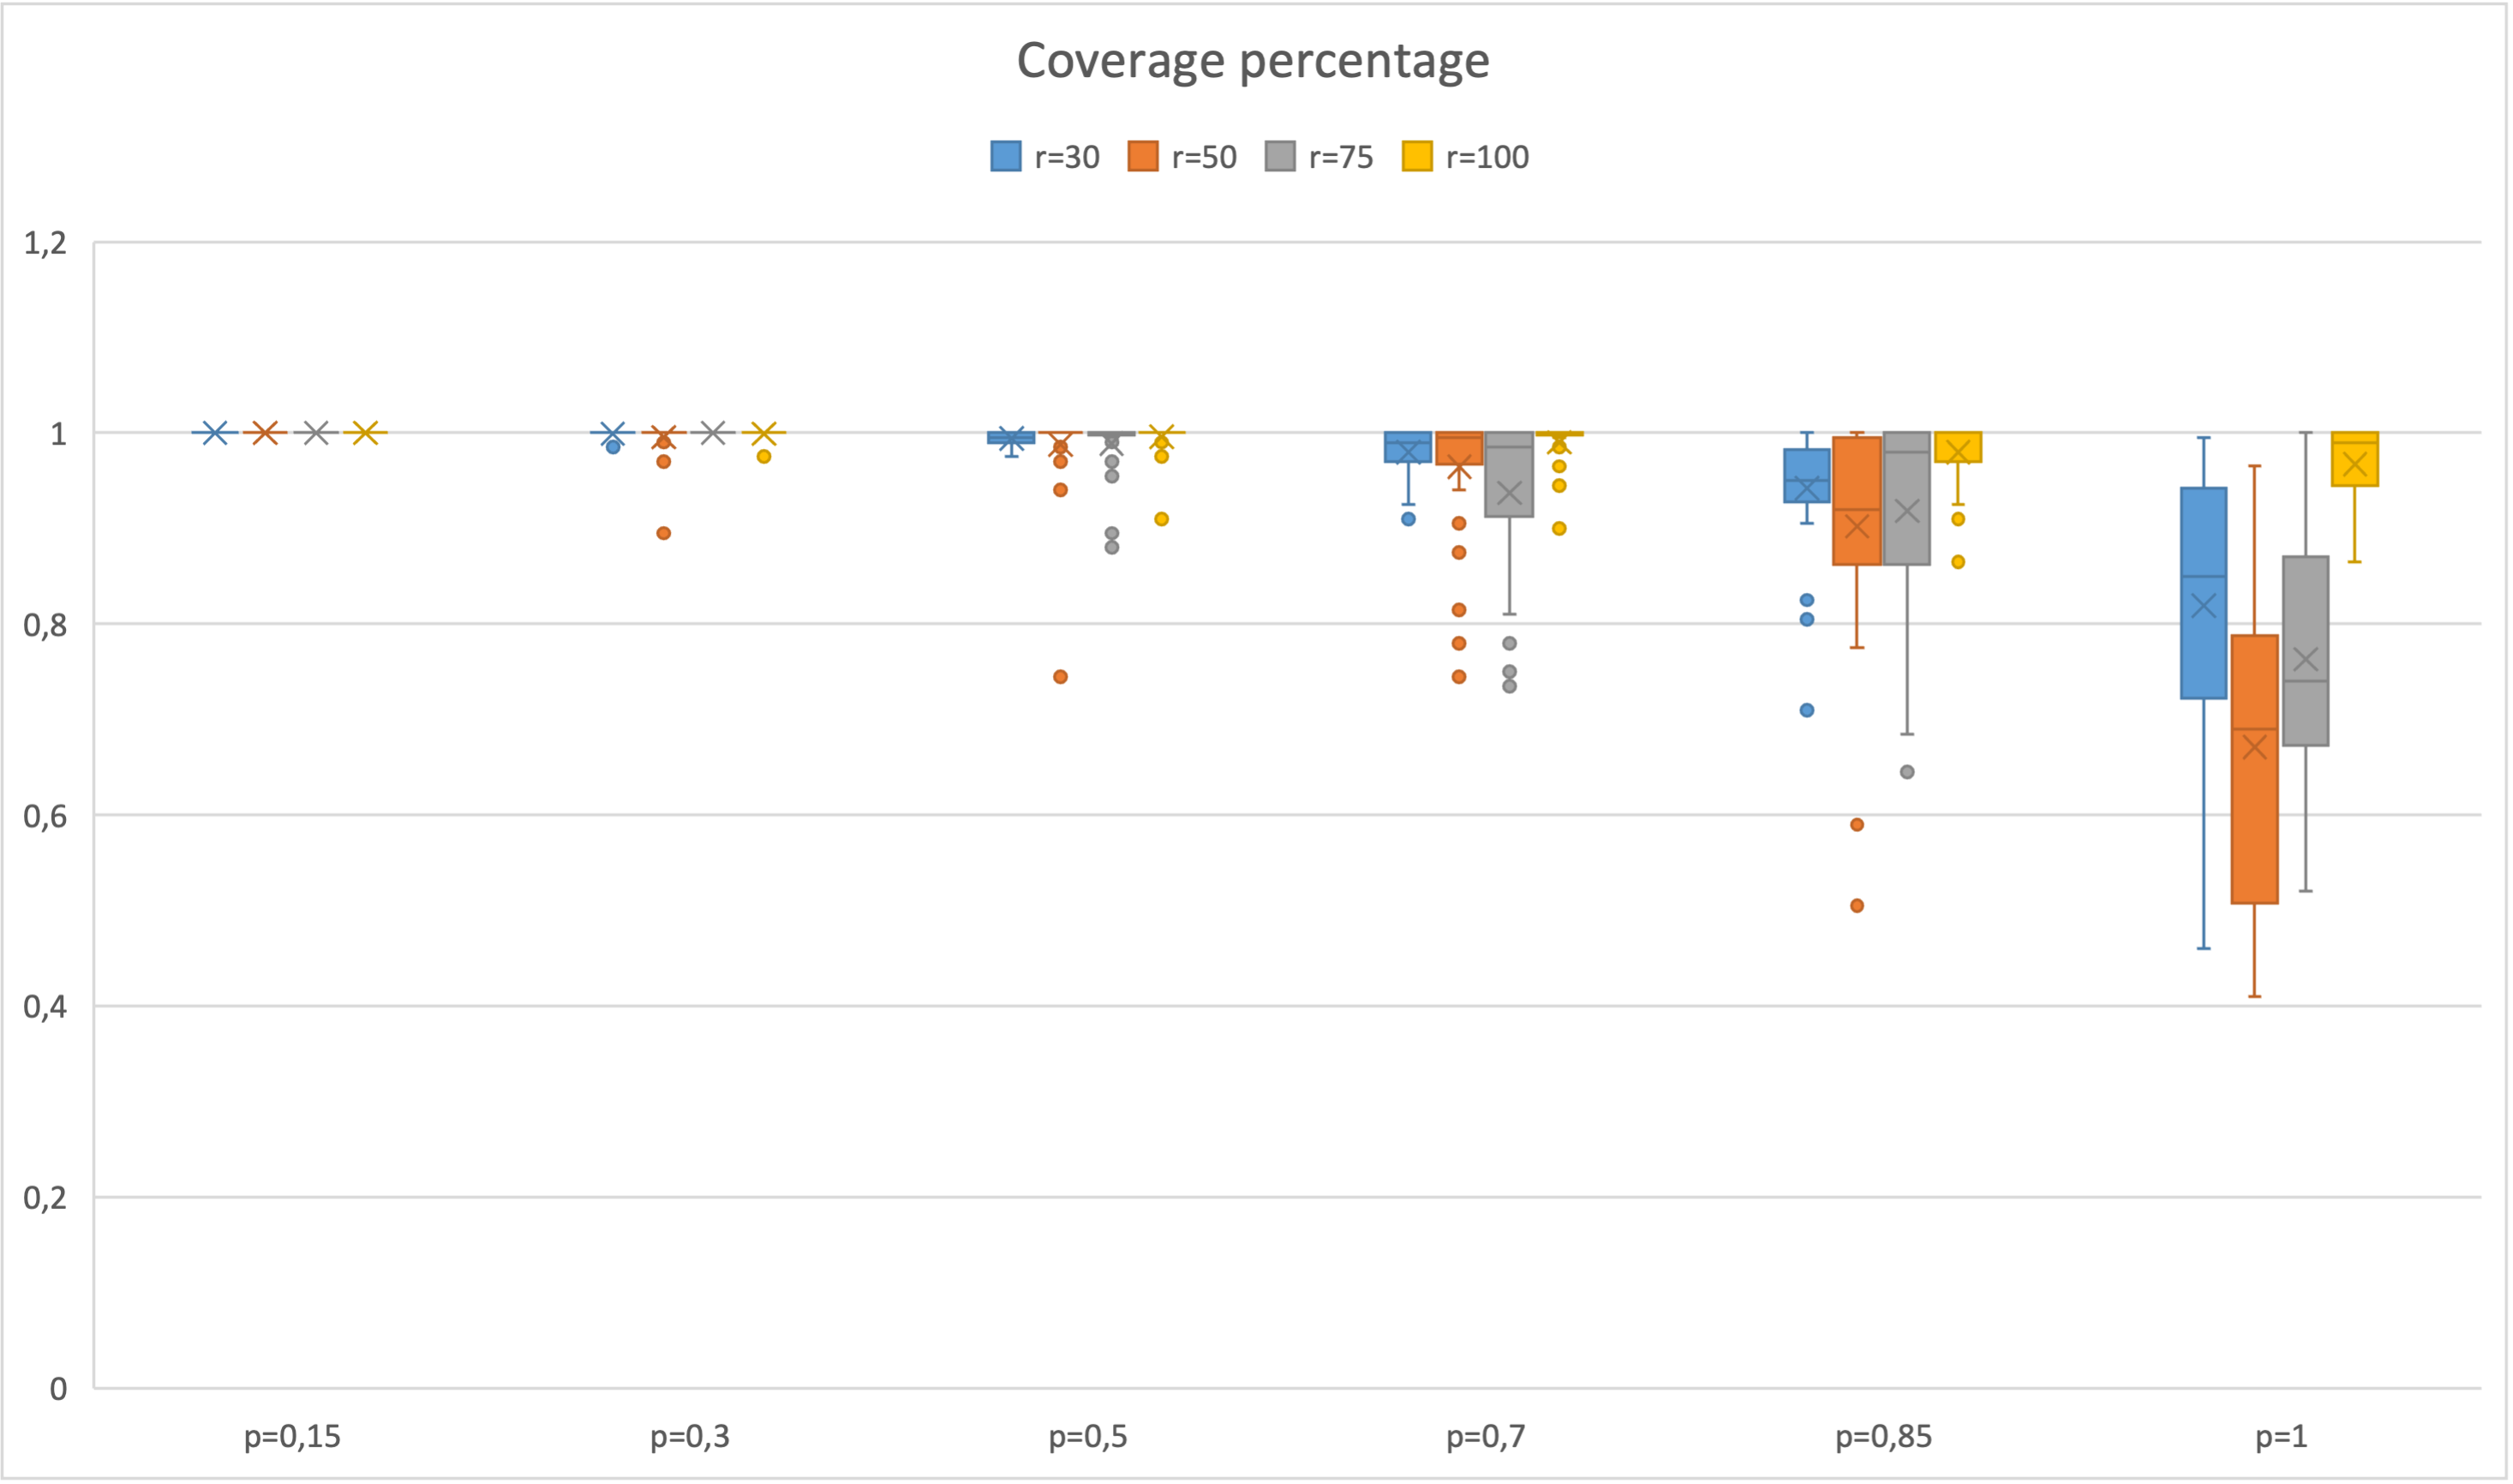
\includegraphics[width= 1\textwidth]{./images/Rate200Boxplot.png}
    \caption{Coverage percentage}
    \label{fig:coverage-percentage}
\end{figure}

\noindent Looking at this graph, it can be seen that increasing the probability does not give better coverage in most cases, as one would expect. In fact, it should be emphasized that as the probability increases, collisions also increase accordingly.

\subsection{Coverage time}
\begin{figure}
\centering
    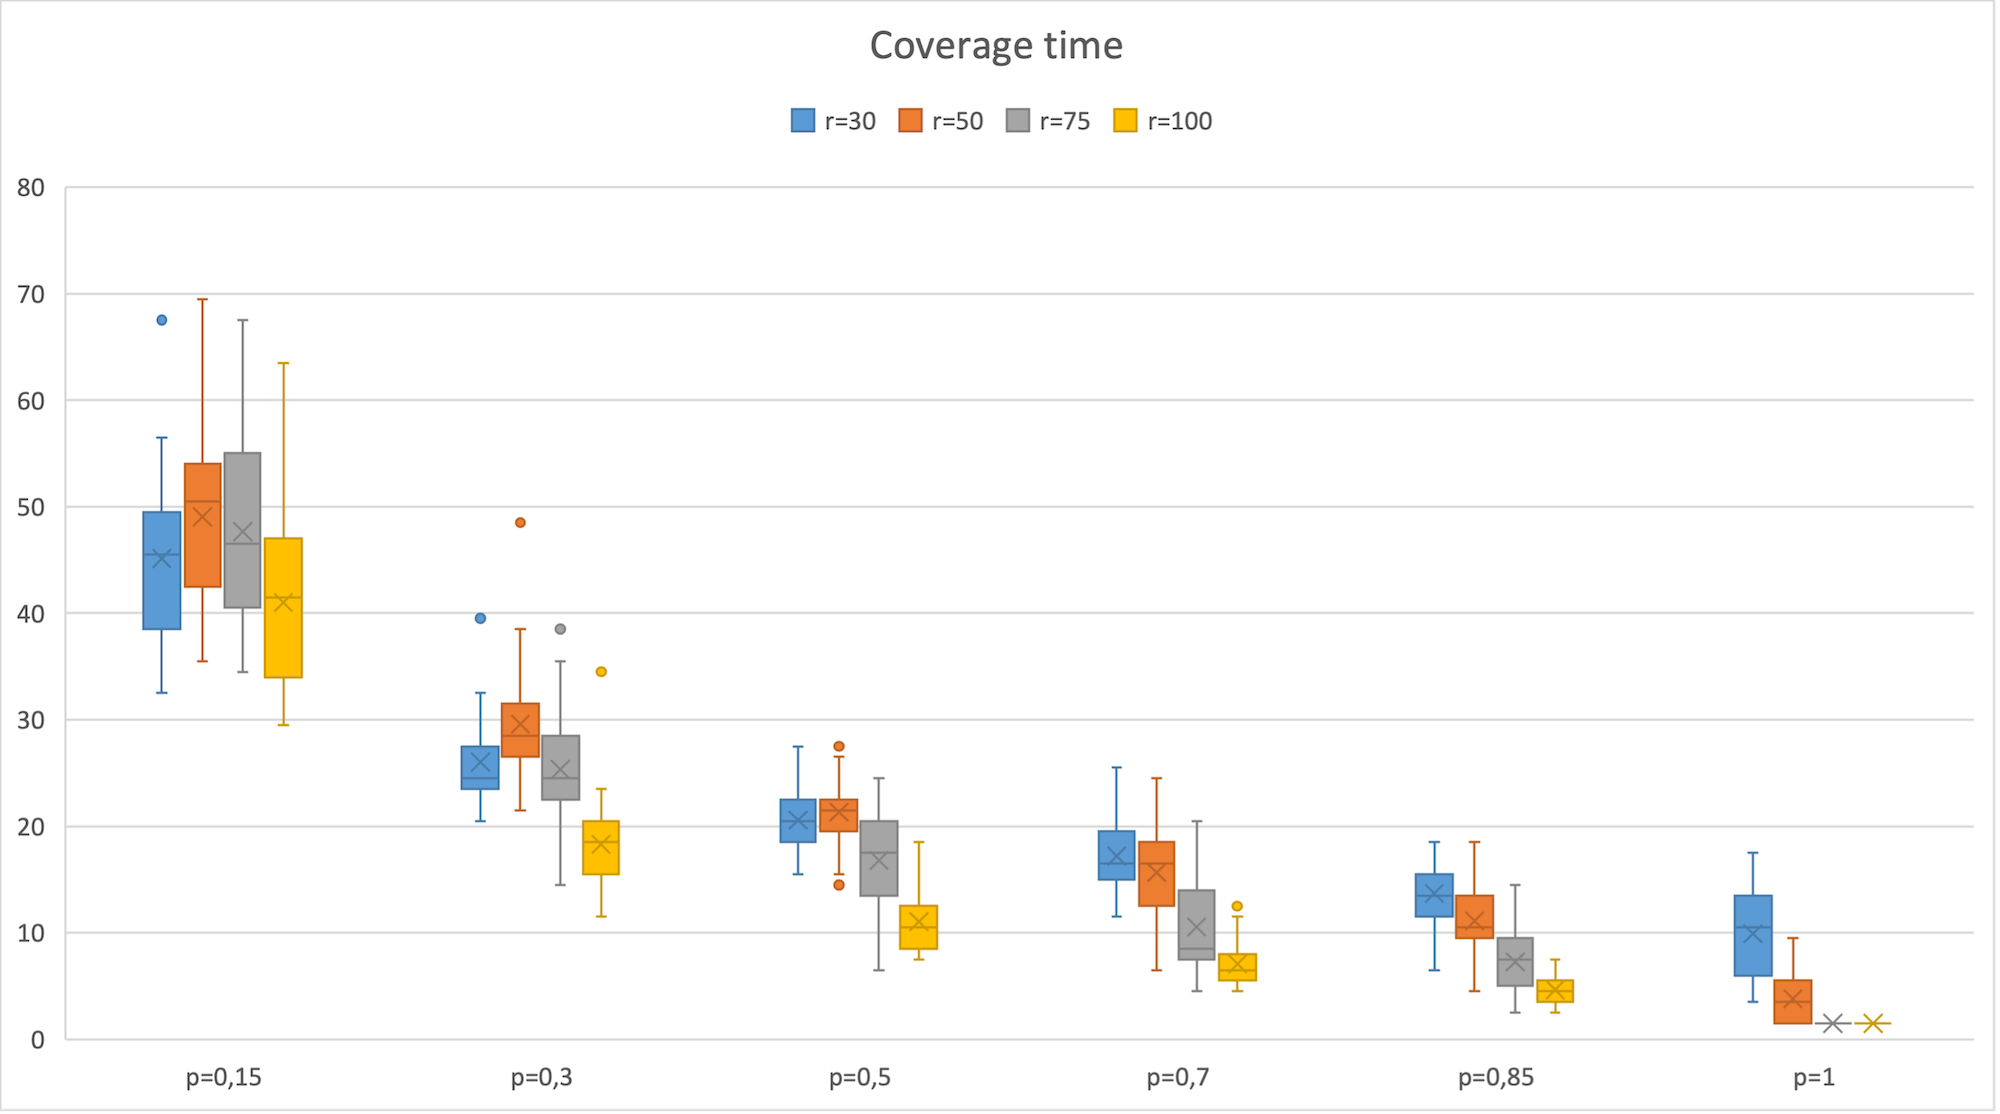
\includegraphics[width= 1\textwidth]{./images/Time200Boxplot.png}
    \caption{Coverage time}
    \label{fig:coverage-time}
\end{figure}
\noindent As imagined, the coverage time decreases as the probability increases, as a higher probability translates into more nodes that can send the infection message.

\subsection{Mean collision rate}

\begin{figure}
\centering
    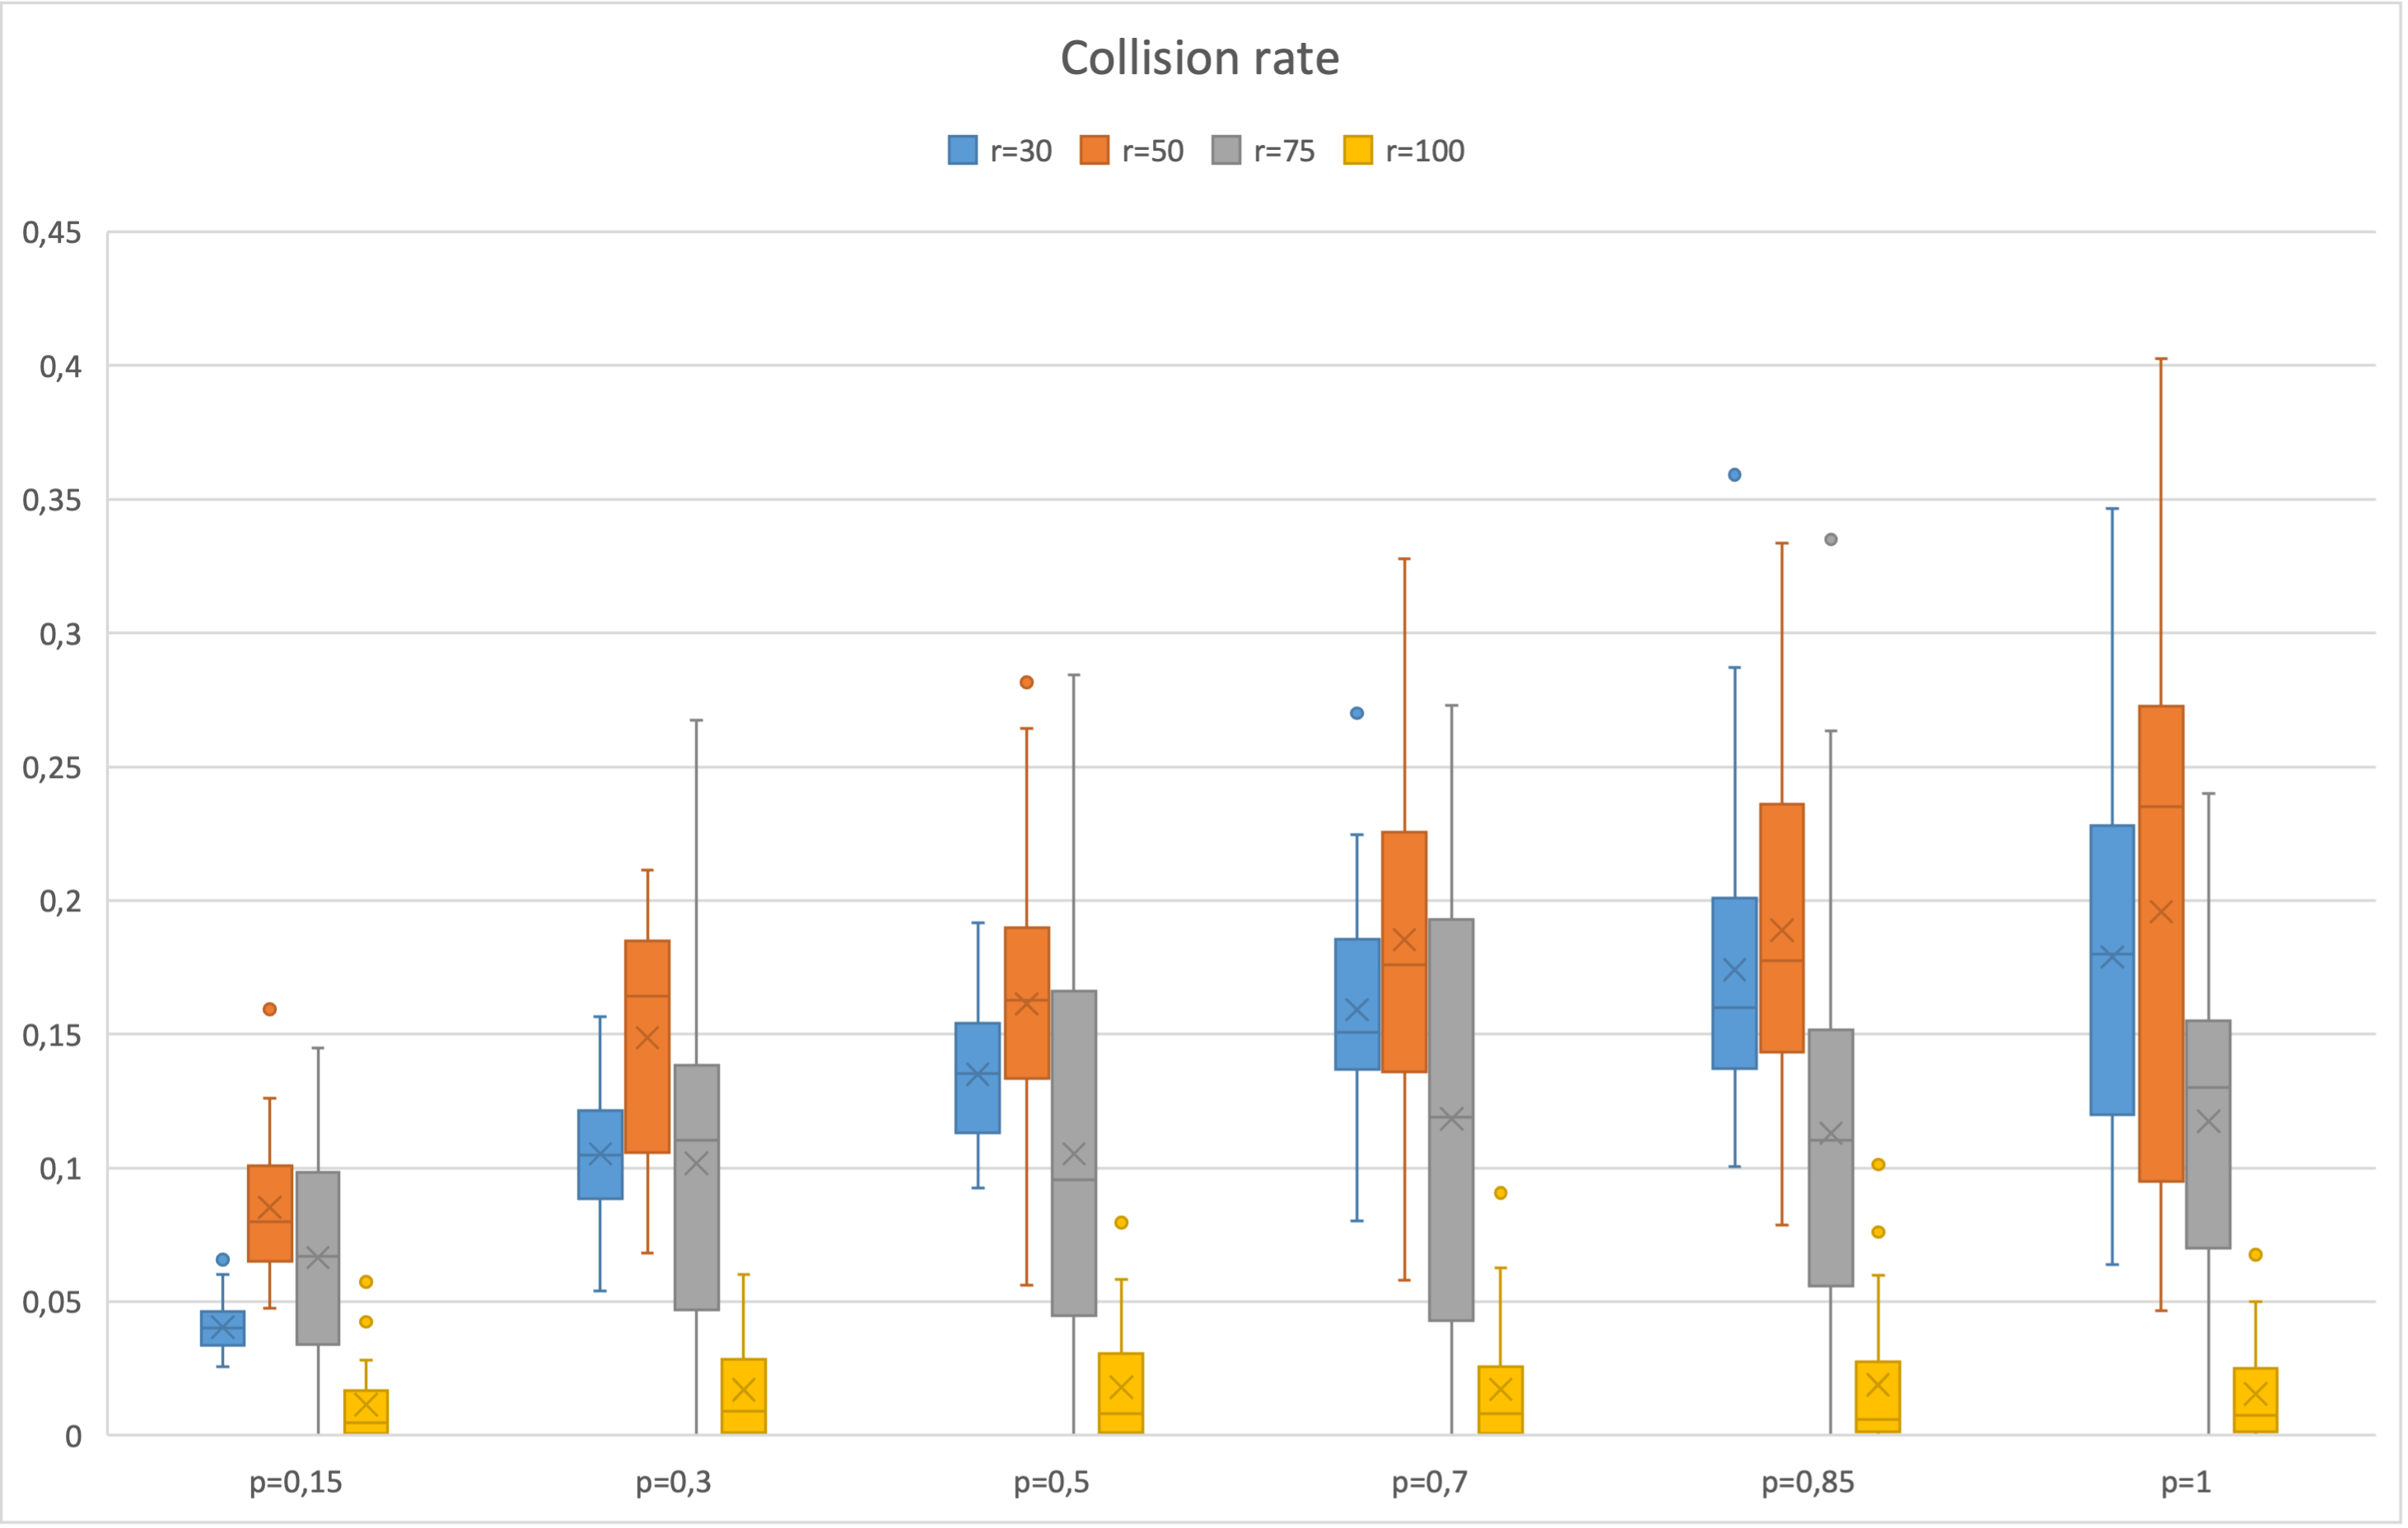
\includegraphics[width= 1\textwidth]{./images/Collision200Boxplot.png}
    \caption{Mean collision rate}
    \label{fig:mean-collision-rate}
\end{figure}

\noindent As regards the collision index, the average value from the initial instant to the completion instant was obtained for all 33 runs. It was not possible to detect clearly visible trends, however, it should be noted that as the radius and the probability increase, the possibility of having many nodes reached by the infection message in the first instants without collisions is high.

\clearpage 

\subsection{Hierarchy of priorities}
Thinking of a real system we have elaborated a hierarchy of priorities to try to understand which system was the most adherent to these characteristics:

\begin{enumerate}
\item High coverage percentage
\item Minimum coverage time
\item Minimum collision rate
\end{enumerate}

Considering runs of interest, as highlighted in Table \ref{tab:run-to-analyze}, we filter only those with $(p=0.15)$ and with $(p=0.3;r=75)$, as they are the only configurations always covering all nodes.
We can rank them based on the coverage time, using Table \ref{fig:coverage-time} and we see that an increase for low probabilities is clearly beneficial for a system speed-up. We can observe that the third quartile for $p=0.3$, $r=75$ is strictly below the first quartile for every configuration with $p=0.15$ and thus we can assert with a confidence level of at least 75\% that this configuration is faster. Therefore we choose it as the best trade-off to analyze.

\subsection{Time evolution}
Thanks to the data collected, we have the state of the system for each instant of time, and we are able to analyze the temporal evolution of the system. In the graph in Figure \ref{fig:done-status} we have considered radius 75 and probabity 0,3 inside the 200 nodes case.
\begin{figure}[H]
\centering
    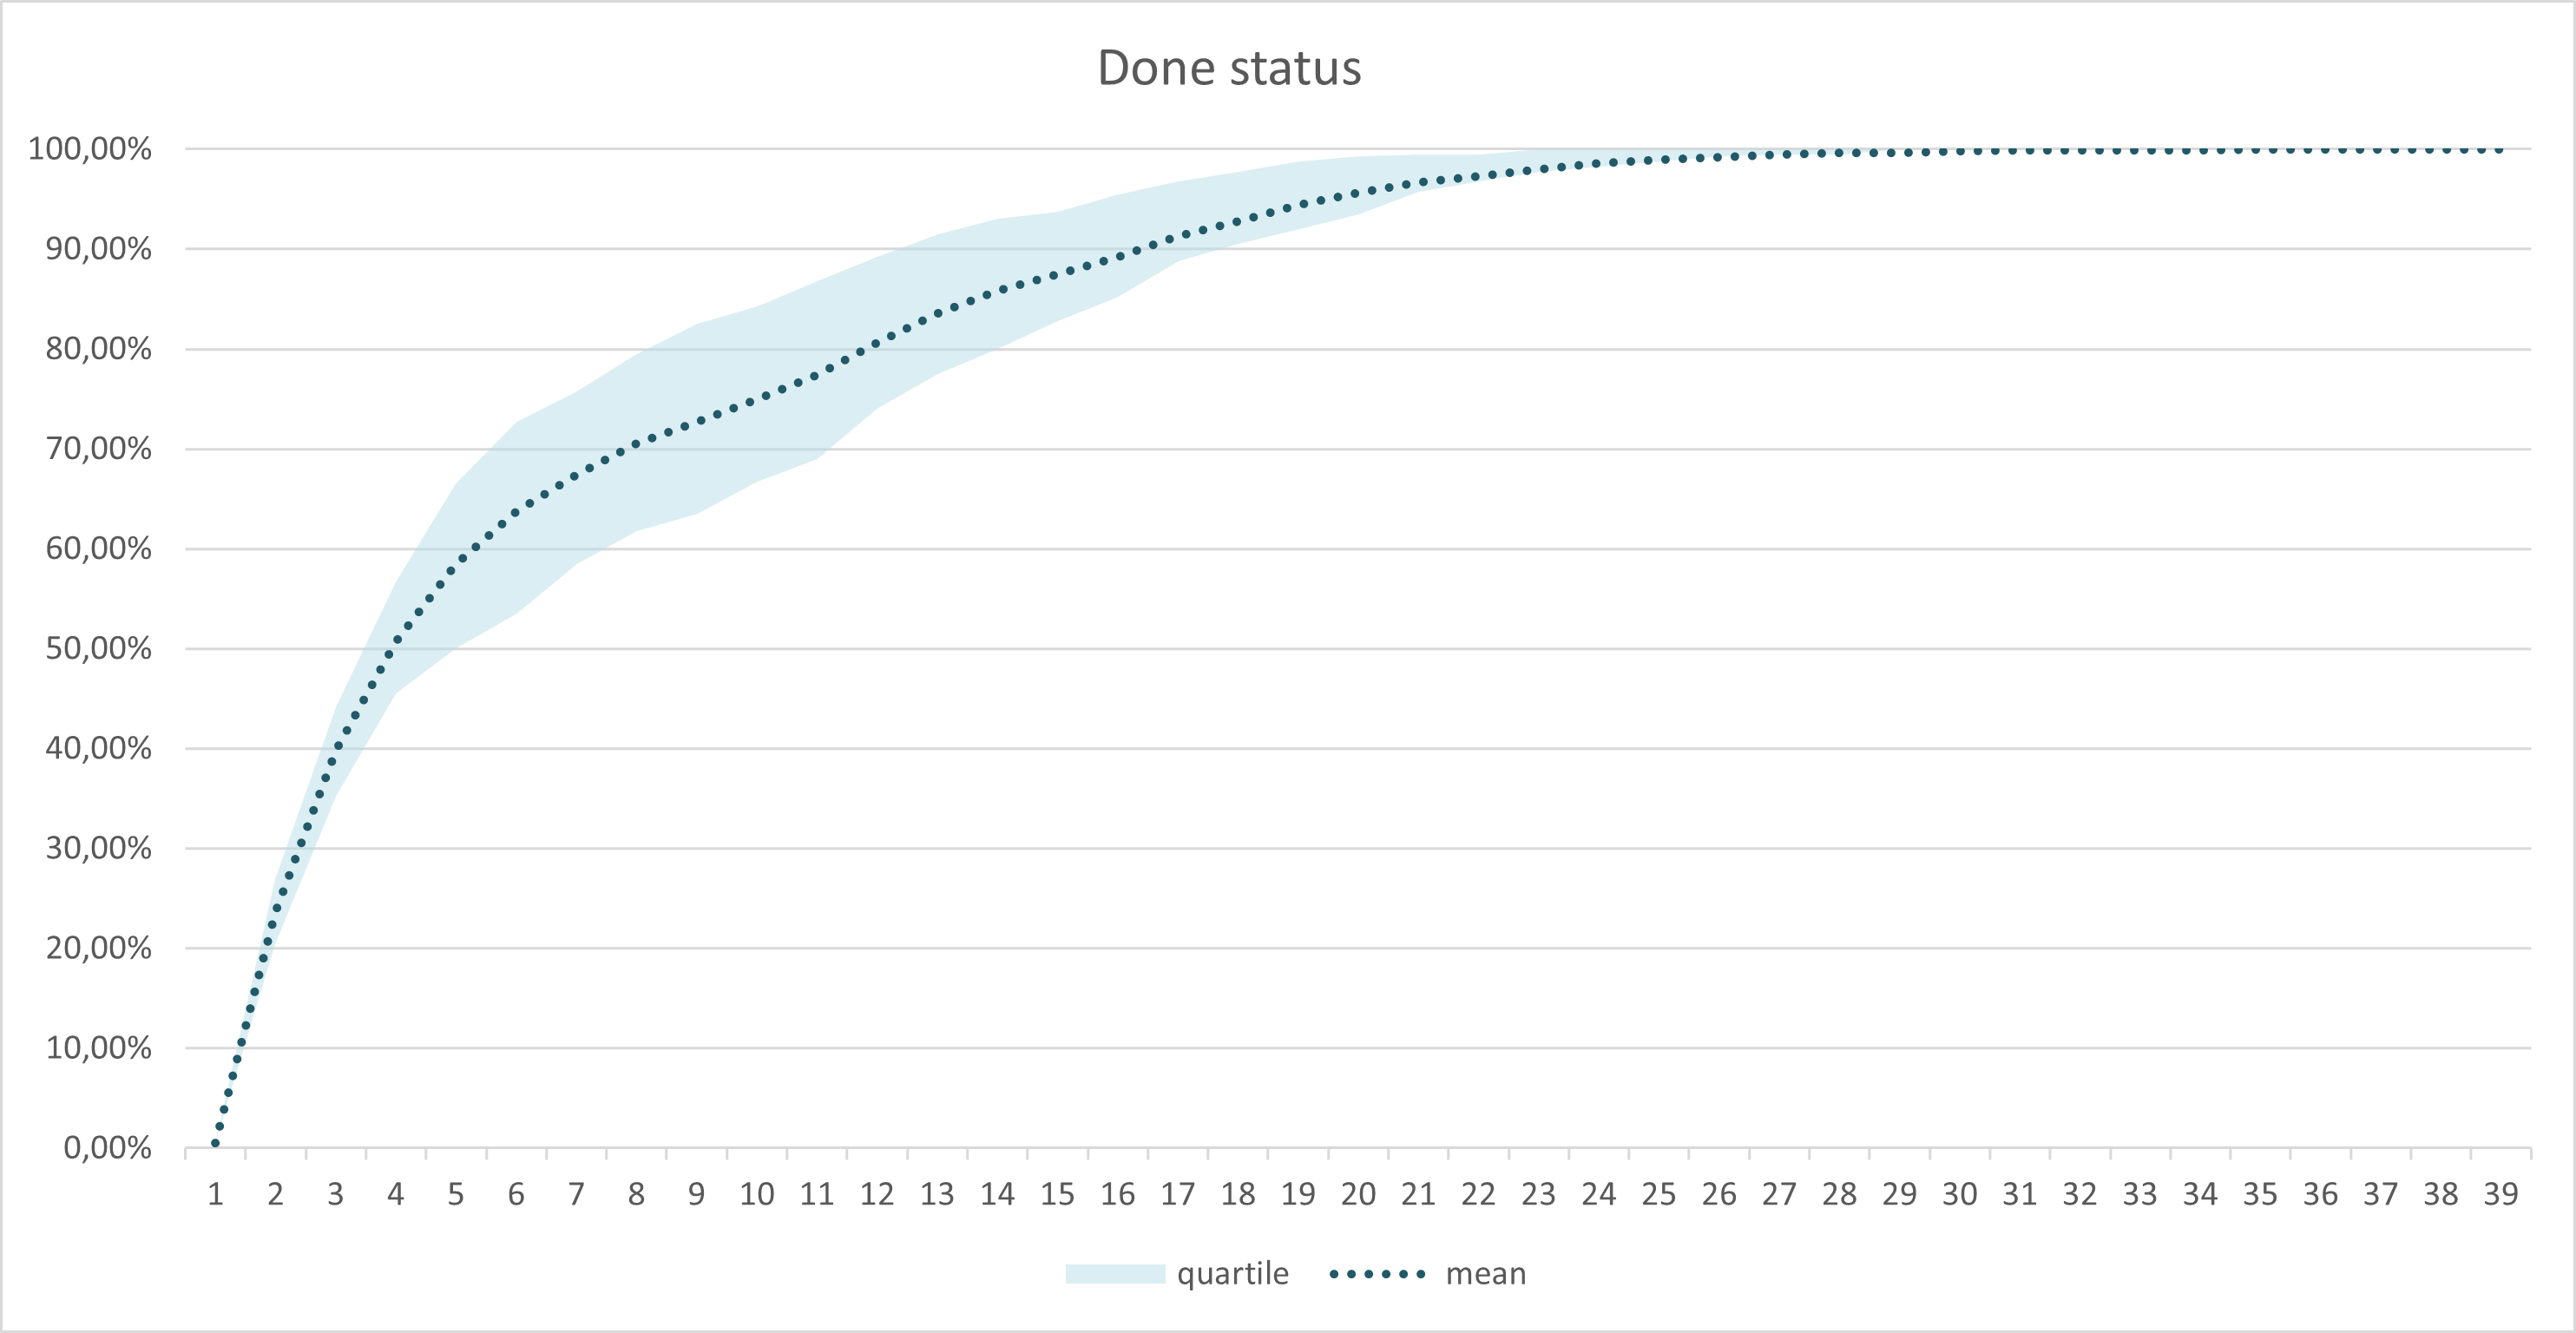
\includegraphics[width= 1\textwidth]{./images/DoneStatus_200N-30p75r.png}
    \caption{Done status}
    \label{fig:done-status}
\end{figure}

\subsection{Factorial Analysis of ending time and ending coverage}

We compute a $2^kr$ factorial analysis to highlight the influence of radius $r$ and probability $p$ on two of our performance indexes, fitting the output variable to a bi-dimensional nonlinear regression model in the form of 
$$
y = q_0 + x_R \cdot r + q_P \cdot p + q_{RP} \cdot r \cdot p
$$

Starting with the final node coverage, i.e. the fraction of nodes in the Done status at the end of simulation, extreme values are shown in Table \ref{tab:extreme-factors-end-coverage} and the final influence in Table \ref{tab:influence-on-end-coverage}

\begin{table}[h!]
\centering
\begin{tabular}{|cl|r|r|l}
\cline{1-4}
\multicolumn{2}{|c|}{\multirow{2}{*}{End Coverage}}     & \multicolumn{1}{c|}{Radius} & \multicolumn{1}{c|}{}   &  \\ \cline{3-4}
\multicolumn{2}{|c|}{}                                  & \multicolumn{1}{l|}{10}     & \multicolumn{1}{l|}{75} &  \\ \cline{1-4}
\multicolumn{1}{|c|}{\multirow{2}{*}{Probability}} & 15 & 0,907273                    & 1                       &  \\ \cline{2-4}
\multicolumn{1}{|c|}{}                             & 85 & 0,57303                     & 0,918333                &  \\ \cline{1-4}
\end{tabular}
\caption{Extreme factor levels for ending coverage}
\label{tab:extreme-factors-end-coverage}
\end{table}

\begin{table}[h!]
\centering
\begin{tabular}{|l|l|l|l|l|l|l|}
\hline
                       & I        & Prob     & Radius   & RP       &          &          \\ \hline
                       & 1        & -1       & -1       & 1        & 0,907273 & 0,003319 \\ \hline
                       & 1        & 1        & -1       & -1       & 0,57303  & 0,076523 \\ \hline
                       & 1        & -1       & 1        & -1       & 1        & 0,022602 \\ \hline
                       & 1        & 1        & 1        & 1        & 0,918333 & 0,004716 \\ \hline
4q                     & 3,398636 & -0,41591 & 0,43803  & 0,252576 &          & 0,107161 \\ \hline
q                      & 0,849659 & -0,10398 & 0,109508 & 0,063144 &          &          \\ \hline
4 q\textasciicircum{}2 &          & 0,043245 & 0,047968 & 0,015949 &          &          \\ \hline
                       &          &          &          &          &          &          \\ \hline
Influenza              &          & 0,403551 & 0,447621 & 0,148828 &          &          \\ \hline
\end{tabular}
\caption{Influence of factors for ending coverage}
\label{tab:influence-on-end-coverage}
\end{table}

We get a pretty balanced influence between radius and probability of about $\sim 42\%$ each, although we must notice that the term $q_P$ is negative $(-0.10)$, which implies a reduction of the final coverage with an increase in probability. Looking at Table \ref{fig:collisions-200} we can clearly understand that this is primarily due to an increase in collisions, which naturally reflects the much lower coverage. Finally, we can assess that the interaction of both parameters is relatively small $(0,1)$, and thus we can study the system by just fixing one parameter and varying the other.

Regarding the completion time, the extreme values are shown in Table \ref{tab:extreme-factors-on-completion-time} and influences in Table \ref{tab:influence-on-completion-time}

\begin{table}[h!]
\centering
\begin{tabular}{|cl|rr|}
\hline
\multicolumn{2}{|c|}{\multirow{2}{*}{Completion Time}}  & \multicolumn{2}{c|}{Radius}                             \\ \cline{3-4} 
\multicolumn{2}{|c|}{}                                  & \multicolumn{1}{l|}{10}       & \multicolumn{1}{l|}{75} \\ \hline
\multicolumn{1}{|c|}{\multirow{2}{*}{Probability}} & 15 & \multicolumn{1}{r|}{111,0152} & 47,65152                \\ \cline{2-4} 
\multicolumn{1}{|c|}{}                             & 85 & \multicolumn{1}{r|}{21,40909} & 7,257576                \\ \hline
\end{tabular}
\caption{Influence of factors for ending coverage}
\label{tab:extreme-factors-on-completion-time}
\end{table}

\begin{table}[h!]
\centering
\begin{tabular}{|l|l|l|l|l|l|l|}
\hline
                       & I        & Prob     & Radius   & RP       &          &          \\ \hline
                       & 1        & -1       & -1       & 1        & 111,0152 & 4119,306 \\ \hline
                       & 1        & 1        & -1       & -1       & 21,40909 & 646,3921 \\ \hline
                       & 1        & -1       & 1        & -1       & 47,65152 & 0,669421 \\ \hline
                       & 1        & 1        & 1        & 1        & 7,257576 & 1566,241 \\ \hline
4q                     & 187,3333 & -130     & -77,5152 & 49,21212 &          & 6332,608 \\ \hline
q                      & 46,83333 & -32,5    & -19,3788 & 12,30303 &          &          \\ \hline
4 q\textasciicircum{}2 &          & 4225     & 1502,15  & 605,4582 &          &          \\ \hline
                       &          &          &          &          &          &          \\ \hline
Influenza              &          & 0,667182 & 0,237209 & 0,09561  &          &          \\ \hline
\end{tabular}
\caption{Influence of factors for ending coverage}
\label{tab:influence-on-completion-time}
\end{table}

It is clear that having both negative coefficients ($q_P = -32.50$ and $q_R = -19.38$) is beneficial for a faster system termination (lower is better). The probability is also $\sim\times 3$ more effective at reducing the completion time, which is also stated by Figures \ref{fig:coverage-time-50}, \ref{fig:coverage-time-200} and \ref{fig:coverage-time-700} and in line with what is expected: even if it means having more collisions, having a higher probability reduces the time a node waits in the Ready status. Again, the interaction of both parameters is negligible and allows us to study the effect of each parameter separately.